
%%%%%%%%%%%%%%%%%%%%%%%%%%%%%%%%%%%%%%%%%%%%%%%%%%%%%%%%%%%%%%%%%%%%%%%%%%%%%
\section{Code tests}
\label{sec.tests}

Ensuring that a complex piece of software is behaving correctly is a
non-trivial task.  While there are a range of techniques that one can
apply to ensure correctness, the \enzo\ code uses two primary methods:
a suite of test problems that can be compared to previous versions of
the code, to ensure that \enzo\ is running correctly on a new
computer, with a new compiler, or after substantial changes have been
made to the code base; and by direct comparisons to other
astrophysical fluid dynamics codes.  We describe the \enzo\ test
methodology in Section~\ref{sec.tests.suite}, code comparisons in
Section~\ref{sec.tests.compare}, and show a small set of
representative test problems in Section~\ref{sec.tests.problems}.  We
further note that the \enzo\ test suite
(Section~\ref{sec.tests.suite}) contains hundreds of test problems, as
well as the ability to compare to a ``gold standard'' solution, and
thus all of the tests shown here are easily reproducible by the
reader.

%%%%%%%%%%%%%%%%%%%%%%%%%%%%%%%%%%%%%%%%%%%%%%%%%%%%%%%%%%%%%%%%%%%%%%%%%%%%%
\subsection{Verifying and validating the \enzo\ code}
\label{sec.tests.vandv}

\subsubsection{The \enzo\ test suite}
\label{sec.tests.suite}

\enzo\ is capable of simulating a large variety of problems types,
with all but a few of these types requiring only a parameter file as an
input.  The notable exception is the cosmology simulation, which takes
as input initial conditions created by other codes.  The suite of test
problems spans a wide range in complexity.  At one end of this spectrum
are simple problems that utilize only a single component of \enzo\ and
for which analytic solutions exist for comparison with the simulation
results.  At the opposite end are problems that exercise a large
portion of \enzo's machinery in concert.  Together, the available
problem types fully cover all of \enzo's functionality.  This enables
them to serve as a vehicle for verifying that the code's behavior
remains stable over time and after modifcation of the codebase.

\enzo\ uses an automated testing framework that allows a user to run,
with a single command, a set of test problems and compare the results
against results produced by any other version of the code.  Within the
\enzo\ source distribution, the test problem parameter files are stored
in a nested directory structure organized according to the primary
functionality tested, e.g., hydrodynamics, gravity, cooling, etc.
Each parameter file is accompanied by a text file containing various
descriptive keywords, such as the machinery tested, the
dimensionality, and the approximate run time.  A test runner script is
responsible for taking as input from the user a series of keywords
that are used to select a subset of all available test problems.  The
test problems are also grouped into three suites: the quick, push, and
full suites, each a superset of the ones named before.  The quick
suite is considered to minimally cover the primary functionality in
\enzo\ and is designed to be run repeatedly during the development
process.  The push suite has slightly increased feature coverage and
is mandated to be run before code changes are accepted into the main
repository.  The full suite consists of all test problems that can be
run with no additional input.  Approximate run times for the quick,
push, and full suite are 15 minutes, 1 hour, and 60 hours,
respectively, on a relatively new desktop computer (circa 2013).

After the test problems are selected by the test runner script, they
are run in succession using either the \enzo\ executable contained
within that distribution or an external executable built from another \enzo\
version and specified by the user.  This allows for any version of the
code to be tested with an identical set of test problems.  After
running the test problem simulations, the test runner then performs a
series of basic analysis tasks using the \texttt{yt} analysis toolkit
\citep{2011ApJS..192....9T, 2011arXiv1112.4482T}.  The default
analysis performed on all test problems includes calculation of
various statistics, such as extrema; mean; and variance, on the fields
present in the output data.  Custom analysis provided by scripts that
accompany the test problem parameter files is run for special cases,
such as when an analytical solution exists that can be compared
against the simulation data.  After the analysis is performed, the
results are compared against a set of gold standard results that are
maintained on a website and downloaded on the fly by the test runner
script.  Alternately, results from any version of \enzo\ can be stored
locally and compared to any other version of the code.  In
Section~\ref{sec.tests.problems}, we describe some of the key test
problems that are used to verify proper behavior.  All of these test
problems, as well as the scripts to generate the figures from them,
are available in the \enzo\ test suite, allowing the interested reader
to regenerate all of the figures in Section~\ref{sec.tests.compare}
using the \textit{'methodpaper'} suite of test problems.

\subsubsection{Code comparisons}
\label{sec.tests.compare}

Over the course of its existence, \enzo\ has been involved in numerous
comparisons with other astrophysical codes used for self-gravitating
fluid dynamics.  In general, \enzo\ behaves in a manner similar to other
grid-based (and particularly AMR-based) codes, as we will summarize below.

\enzo\ has been involved in multiple cosmological code comparisons,
including the Santa Barbara Cluster code comparison project
\citep{SantaBarbara}, a large comparison of N-body simulations
\citep{2008CS&D....1a5003H}, as well as several direct comparisons
between \enzo\ and the GADGET SPH code under a variety of
circumstances, including N-body and adiabatic hydrodynamics
\citep{2005ApJS..160....1O,2005MNRAS.364..909V, 2011MNRAS.418..960V}
and simulations of the Lyman-alpha forest \citep{2007MNRAS.374..196R}.
The \enzo\ code typically has a more difficult time resolving
small-scale self-gravitating structures (for an equivalent dark matter
particle count and nominally equivalent force resolution), but does
comparably well as a tree-based code for larger structure, and is
typically superior in terms of resolving fluid features due to its
higher-order (and artificial viscosity-free) Piecewise Parabolic
Method hydrodynamics solver.  When examining classical test cases such
as the Santa Barbara project \citep{SantaBarbara}, \enzo\ forms galaxy
clusters with very similar density, temperature, and entropy profiles
to other grid-based codes that use Godunov-type hydro methods, which
systematically differed from particle-based codes using SPH in this
code comparison.  Similarly, in galaxy cluster simulations that look
specifically at the properties of cosmological shocks
\citep[e.g.][]{2011MNRAS.418..960V}, \enzo\ produces results that are
similar to other high-order grid-based hydrodynamics codes, and far
superior performance of \enzo\ is observed (in terms of resolution of
fluid features and shock detection) in low-density regions when
compared to a particle-based code.  In tests of the Lyman-alpha forest
that include radiative cooling and a uniform metagalactic ultraviolet
background, \enzo\ and Gadget provide results on metrics such as the
matter power spectrum that are comparable to within 5\%
\citep{2007MNRAS.374..196R}.

Several comparisons have been made that focus specifically on
hydrodynamics solvers and fluid behavior.  In particular, the work of
\citet{2007MNRAS.380..963A} and \citet{Tasker2008} perform
head-to-head comparisons between several grid- and particle-based
codes for a variety of fluid-centric test problems (including shocked gas clouds,
self-gravitating, translating clouds, and Sedov-Taylor explosions),
and show that \enzo\ is comparable or superior in behavior to the
other grid-based hydrodynamics codes involved in the comparison, and
provide useful information on the sort of practical challenges that a
user of an
AMR code such as \enzo\ may experience.  More specific comparisons, including one
specifically testing the linear and nonlinear growth of the
Kelvin-Helmholz instability \citep{2012ApJS..201...18M}, as well as a
comparison that more
broadly examines Galilean invariance in grid-based codes
\citep{2010MNRAS.401.2463R}, show that \enzo, and in particular its
implementation of the Piecewise Parabolic Method hydrodynamics solver,
converge to the correct solution as expected, and generally provide
less diffusive solutions than lower-order codes, including those that
use artificial viscosity.  Finally, two code comparison projects have
been undertaken to examine turbulence in hydro codes -- one studied
the behavior of decaying isothermal supersonic turbulence
\citep{2009A&A...508..541K}, and the other looked at supersonic
magnetohydrodynamical turbulence \citep{2011ApJ...737...13K}.  Both
included the \enzo\ code, with the former testing the PPM
hydrodynamics and the latter the constrained transport MHD
implementation of \citet{Collins10}.  In both cases, \enzo\ performed similarly to other
grid-based codes that use Godunov-based fluid solvers, and typically
had better effective resolution than particle-based codes using the
same number of particles as the \enzo\ simulation used grid cells.

Three other comparisons between the \enzo\ code and other simulation
tools have been performed that focus on physics other than gravity and
fluid flow.  The flux-limited diffusion radiation transport scheme was
measured against several test problems by \citet{IlievEtAl2009},
producing results that are similar to both expected results (i.e.,
analytic test problems) and other methods (i.e., codes using other
methods, written by other groups), although there are some minor
differences (although all codes in the study exhibited differences
from the majority of other codes on at least a subset of the tests).
\citet{2011ApJ...726...55T} shows the results of varied reaction rate
coefficients for the formation of molecular hydrogen via the 3-body
process in both the \enzo\ and Gadget-2 codes.  Similar trends were
visible in both the \enzo\ and Gadget simulations, though at a
nominally equivalent resolution (i.e., with particle and cell gas
masses being comparable) \enzo\ simulations typically displayed a
substantially higher level of gas structure.  This is unsurprising due
to \enzo's higher-order hydro solver.  Finally,
\citet{2012ApJ...744...52P} show the results of comparing \enzo\ in
its non-AMR mode to a smoothed-particle hydrodynamics code, SNSPH, in
the context of common-envelope binary stellar interactions.  The
authors show that the codes display reasonable convergence properties
as a function of simulation resolution, and also agree quite well with
each other -- however, the observed mass-loss rates do not agree
particularly well with observations.

%%%%%%%%%%%%%%%%%%%%%%%%%%%%%%%%%%%%%%%%%%%%%%%%%%%%%%%%%%%%%%%%%%%%%%%%%%%%%
\subsection{Representative test problems}
\label{sec.tests.problems}

The \enzo\ test suite (described in Section~\ref{sec.tests.suite})
contains hundreds of test problems that probe the code's behavior in a
wide range of physical circumstances, and explicitly test each physics
package in the \enzo\ code, both individually and in combination.  It
is impractical to include a substantial fraction of these problems in
a method paper; as a result, we have chosen to publish the results of
only a small subset of particularly crucial test problems here.  If
the interested reader desires, they can download \enzo\ and
\texttt{yt}, run the test suite, and see the results of any other test
problem and its comparison to an analytic solution (if available).

The general structure of each test problem description is as follows.
We will describe the construction of the test problem (including its
initial and boundary conditions), the analytical or expected
solutions, and motivate why we have included it in the paper.  After
that, we will show and describe \enzo's solution to the test problem.

% General structure for each test problem: Outline how the test problem
% is constructed (initial and boundary conditions), the analytical
% solution, why we have in the paper (what does it break, or what flaw
% does it expose (not in enzo of course)), a plot showing how well enzo
% solves said test problem, and a brief description of the plot and how
% awesome enzo is.

%%%%%%%%%%%%%%%%%%%%%%%%%%%%%%%%%%%%%%%
\subsubsection{Sod Shock Tube}
\label{sec.tests.sodshock}

We begin the paper test suite with the classic Sod shock tube problem
\citep{Sod78}, which provides a good test of a hydrodynamical solver's
ability to resolve a clean Riemann problem with clear separation
between the three waves.  These waves include a rarefaction fan, a
contact discontinuity, and a moderate shock.  The initial state is 
$\rho_{\rm L}, P_{\rm L} = 1.0, 1.0$ on the left of the boundary at 
$x=0.5$ and $\rho_{\rm R}, P_{\rm R} = 0.125, 0.1$ on the right.
All velocities are initially zero.  In
Figure~\ref{fig.sodshocktube}, we show the density solution at the
final time ($t=0.25$) for three of our hydro solvers -- the spatially third-order
PPM, as well as the two second-order \zeus\ and MUSCL schemes.  We use
100 cells across the domain, (which is a relatively standard choice in
code method papers) and show solutions both with and without adaptive
mesh refinement.  Without AMR (in the top row of the figure), it is
clear that the PPM scheme produces by far the cleanest solution, with
all wave families crisply reproduced (in particular, the contact
discontinuity and shock).  \zeus\ and MUSCL produce similar results,
with MUSCL doing a slightly better job on the rarefaction fan.  In the
figure, we also show the mean absolute deviation from the exact
solution ($||E_\infty||$), as well as the maximum deviation
($||E_1||$).  These numbers confirm the qualitative differences noted
previously.

We also run the same simulation but with two levels of AMR (using a
refinement factor of 2), triggered based on a normalized slope greater
than 10\% in the density.  This refinement criterion results in only
the refinement of strong gradients, and
does not include the rarefaction fan at late times.  The results are
shown in the bottom row of Figure~\ref{fig.sodshocktube}.  Using AMR,
the results are much better for all three methods, with much sharper
shocks and contact discontinuities and even a better representation of
the rarefaction wave, which is only refined beyond the root grid at
early times.  Although the results are improved for all methods, PPM
still produces the best result, as is shown clearly by the computed
error norms (displayed again in each of the individual panels).

\begin{figure}
\begin{center}
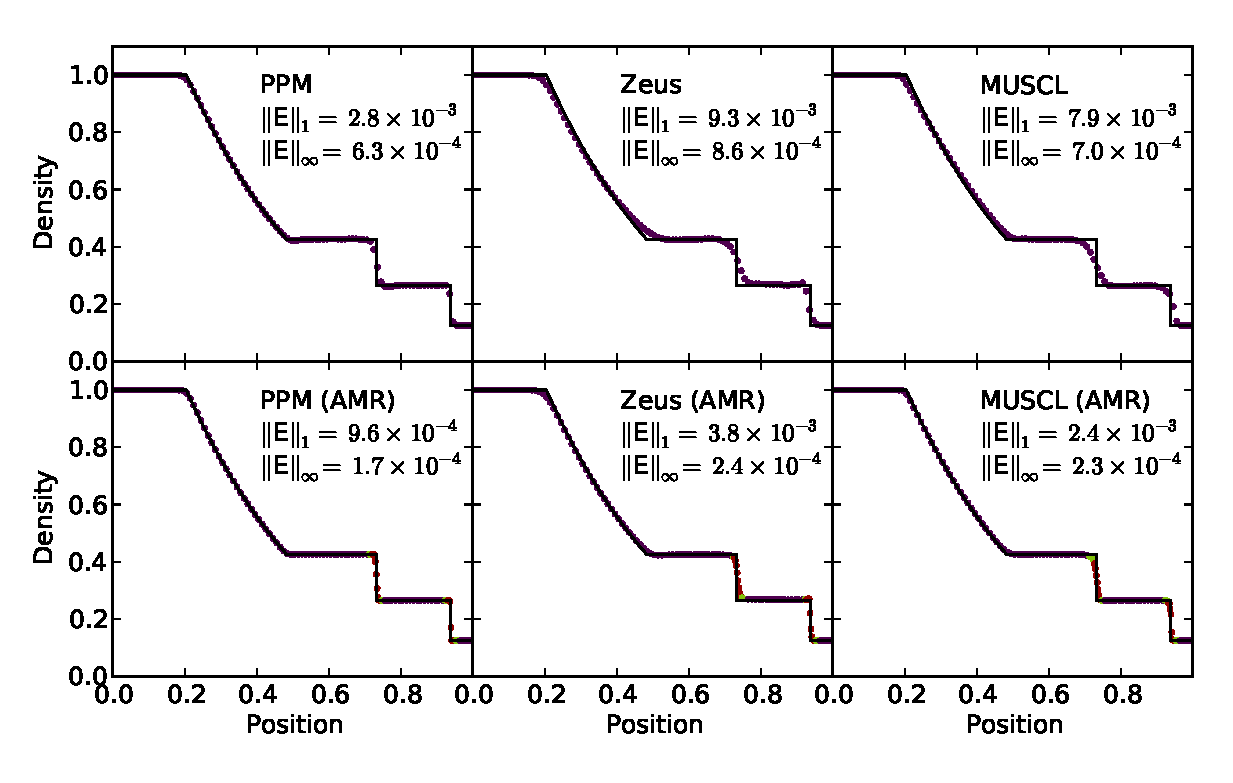
\includegraphics[width=\textwidth]{figures/SodShockTube.eps}
\caption{The density distribution of the classic Sod Shock Tube for
three different solvers (from left to right column) and with (bottom
row) and without (top row) AMR.  In each case 100 zones are used on
the root level and the results are shown at $t=0.25$.  All cells are
plotted and color-coded by level (at the time shown, only small region
surrounding the contact discontinuity and the shock are refined).  In
each panel, we show the analytic solution as a solid line and the $E_1$
and $E_\infty$ error norms in the upper right.}
\label{fig.sodshocktube}
\end{center}
\end{figure}


%%%%%%%%%%%%%%%%%%%%%%%%%%%%%%%%%%%%%%%
\subsubsection{Wave pool}
\label{sec.tests.wavepool}

In this one-dimensional test, we pass a short wavelength, linear wave through a static refined region.  The full domain is from 0 to 1 and the refined region is set from 0.25 to 0.75 at all times.  We modify the left boundary consistent with a single linear sound wave with density given by $\rho(x,t) = \rho_0 (1 + A \sin(kx - \omega t))$, where the amplitude is $A = 0.01$ and the wavelength $\lambda = k/2\pi = 0.1$, and similar expressions exist for the pressure and velocity.  The initial, unperturbed density and pressure are set to unity and we adopt $\gamma = 1.4$.  The (unrefined) root grid is covered with 100 cells, resulting in a wavelength for the linear wave of only 10 cells.  This is, therefore, a challenging problem for hydro methods.  We are particularly interested in any reflection or artifacts introduced by the wave entering and exiting the refined regions.

Figure~\ref{fig.wavepool} shows the evolution of the wave at three different times ($t = 0.2, 0.3$ and 0.8) for three of our solvers (PPM, Zeus, and MUSCL).  The leftmost column show the wave just before it enters the refined region so that we can gauge how the solver is operating in the absence of AMR, the center column shows the wave after it has fully entered the refined region, and the rightmost column shows the wave well after it has exited the refined region.

Beginning with the PPM, we see that even before it has entered the refine region, the wave is slightly damped, which is not unexpected for such a short wavelength mode, even for PPM.  The remaining panels demonstrate that the wave cleanly enters and exits the refined region.  No significant reflection is seen, either on entry or exit, and the amount of damping is mild.

For the Zeus solver, we see that even before it has entered the refined region, there are small oscillations excited behind the wave; although it is also worth noting that the wave itself is beautifully propagated without significant damping or phase errors.  In this test, we use only our standard, low amount of quadratic artificial viscosity -- these waves can be damped by additional viscosity, but we do not add any in order to be sensitive to any artifacts at the grid boundary.  The remaining panels show that the trailing oscillations continue, but do not generate any additional noise -- the end result is similar to the case without any refined region.

Finally, the MUSCL solver shows also shows a very clean entry and exit from the refined region without any oscillations, although (for the PLM reconstruction used here) the wave is spread more than with the other methods.

\begin{figure}
\begin{center}
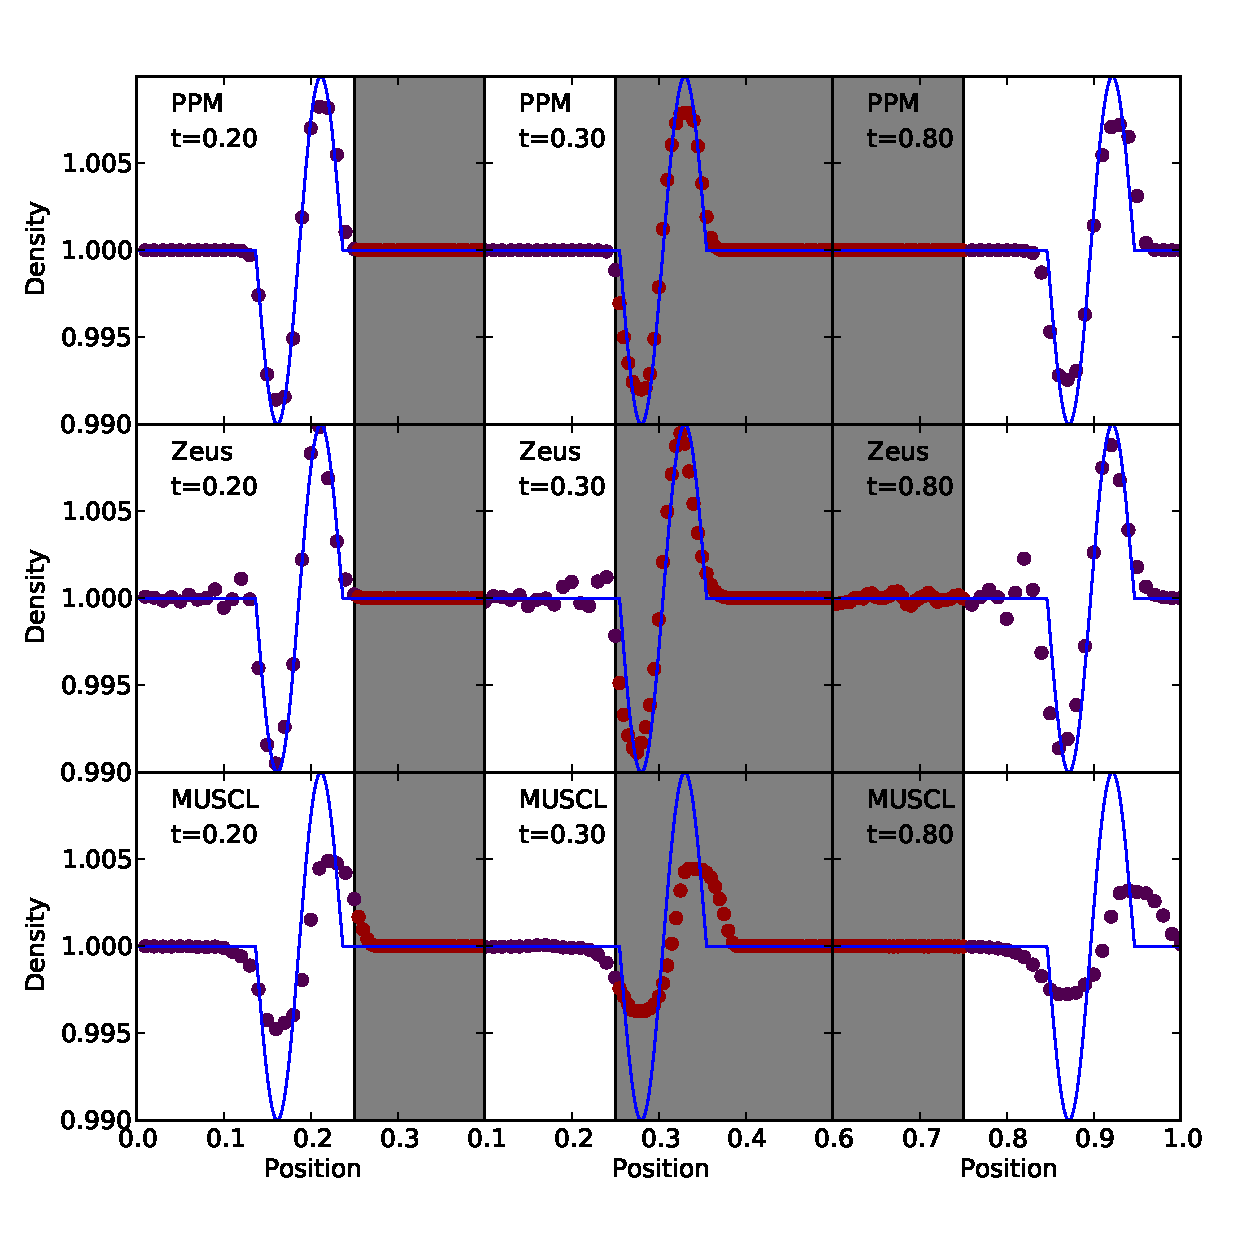
\includegraphics[width=0.8\textwidth]{figures/WavePool.eps}
\caption{This plot shows, for each column, three snap shots (at $t=0.2, 0.3$ and 0.8) of a linear wave as it propagates through the grid.  The static refined region extends from $x = 0.25$ to 0.75 and is shown in grey in each panel.  The individual cells are also color-coded by level: blue indicates the root grid, and red is for the refined region.  Each row shows the result for a different solver (top is PPM, middle is Zeus, and the bottom is MUSCL).   The solid line shows the analytic solution for a linear, undamped wave.  Note that we focus each panel on a small region of the entire domain to better show the wave itself.}
\label{fig.wavepool}
\end{center}
\end{figure}

%%%%%%%%%%%%%%%%%%%%%%%%%%%%%%%%%%%%%%%
\subsubsection{Shock pool}
\label{sec.tests.shockpool}

The next problem is similar to the last one, but examines how a shock wave with a Mach number of 2 passes into and out of a static refined region (again defined from $z=0.25$ to 0.75).  The density and pressure in the domain is initially set equal to 1.0, with zero velocity, and then at $t=0$, the left boundary is set with the density, pressure and velocity appropriate for $M=2$ shock wave.

In Figure~\ref{fig.shockpool}, we show the evolution of the shock wave at three times, again corresponding to just before entering the refine region (left column), after entering the refined region (center), and after exiting the refined region (right).  We examine the same set of three solvers as in the previous test problem.

Beginning with PPM (top row), we see that this method captures the shock in a small number of zones with only a small amount of oscillation.  Open entering the refined region, the shock finds itself broader than the natural width of the scheme (since the cell spacing is decreased by a factor of 2), and so the shock front contracts, causing a slight entropy perturbation in the post-shock gas. 

For Zeus (middle row of Figure~\ref{fig.shockpool}, the shock is broadened because of artificial viscosity, and there are slightly more post-shock oscillations, although again quite mild.  The impact of entering and exiting the refined region is somewhat larger than in PPM; however, the most noticeable difference is the incorrect position of the shock front, which is due to the fact that the scheme is not energy-conserving (see also the Sedov problem, below), and has essentially nothing to do with the passage through the refined region.

Finally, the MUSCL scheme produces a shock which is intermediate in width between the two previous cases.  This method is energy conserving and so correctly reproduces the shock speed.  The oscillations are mild except for the cell immediately outside of the refined region upon exiting.

\begin{figure}
\begin{center}
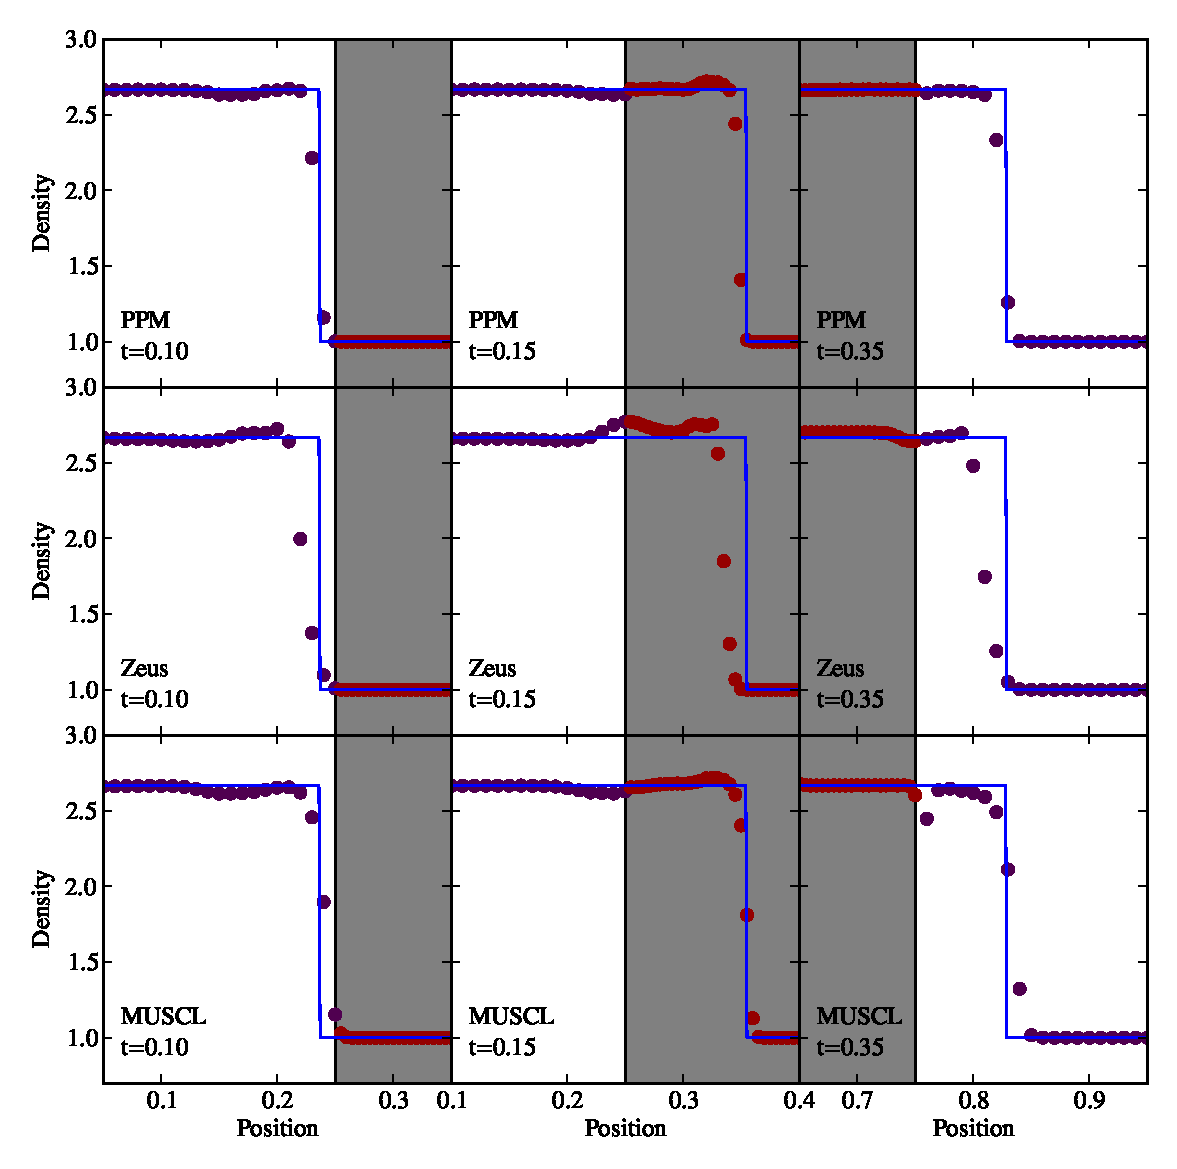
\includegraphics[width=0.8\textwidth]{figures/ShockPool}
\caption{This plot shows, for each column, three snap shots (at $t=0.1, 0.15$ and 0.35) of a $M=2$ shock wave as it propagates through the grid with a static refined region extends from $x = 0.25$ to 0.75 (shown in grey in each panel).   Each row shows the result for a different solver (PPM/Zeus/MUSCL from top to bottom).  The solid line shows the analytic solution.  Note that we focus each panel on a small region of the entire domain to better show the shock front.}
\label{fig.shockpool}
\end{center}
\end{figure}

%%%%%%%%%%%%%%%%%%%%%%%%%%%%%%%%%%%%%%%
\subsubsection{Double mach reflection}
\label{sec.tests.doublemach}

The double mach reflection test is a classic two-dimensional test of
hydrodynamic algorithms, and was originally described in
\citet{1984JCoPh..54..115W} \citep[and more recently
in][]{2008ApJS..178..137S}.  In this problem, shown in
Figure~\ref{fig.doublemach}, a shock is injected at an angle to a
reflecting surface (the -y boundary), and a jet appears along the
reflecting surface.  The ideal solution is self-similar, and the
appearance of this solution is highly sensitive to numerical
diffusion.  If numerical noise is present, a Kelvin-Helmholz
instability develops along this jet and breaks the self-similarity.

In the test problem shown in Figure~\ref{fig.doublemach}, a 2D
simulation with $960 \times 240$ cells was formed with a domain of $x
= [0, 4]$ and $y = [0, 1]$.  We use an ideal gas equation of state of
$\gamma = 1.4$, a pre-shock density of 1.4, and a pre-shock specific
internal energy of $2.5/1.4$ (all in arbitrary units).  A Mach 10
shock is initialized with a shock normal that is 30$^\circ$ from the
x-axis and an initial position on the lower boundary of x$ = 1/6$.
The lower y boundary and right x boundary are reflecting; the left x
boundary is inflowing, and the upper y boundary has a time-dependent
boundary condition that allows the shock to propagate into the domain
as if it extends to infinity.  The simulation starts at t$ = 0$ and
runs until t$ = 0.205$ (arbitrary units), at which point the rightmost
extent of the shock should be at roughly x$ = 3$.  In this run, we use
the direct Eulerian implementation of the piecewise parabolic hydro
method, with the diffusion, flattening, and shock steepening all
turned on.

It is instructive to compare Figure~\ref{fig.doublemach} to Figure 9
in~\citet{1984JCoPh..54..115W}.  By the end of the simulation, a dense
jet is apparent at the leading edge of the shock, propagating along
the x-axis.  The shape of this jet is sensitive to numerical
diffusion, and our figure compares favorably to the higher-order
images from Woodward \& Colella.

\begin{figure}
\begin{center}
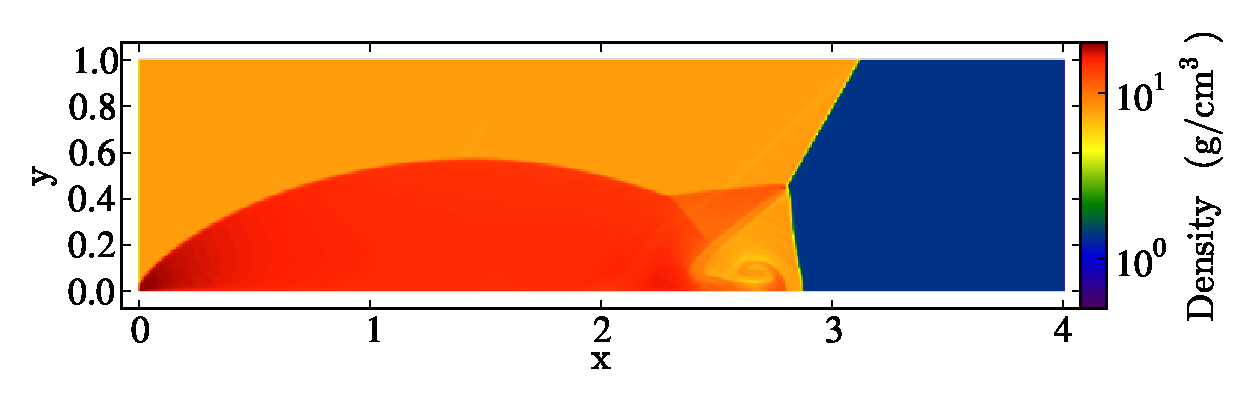
\includegraphics[width=0.8\textwidth]{figures/DoubleMachTest.eps}
\caption{Density field at the final time in the Double Mach test.  A
Mach 10 shock is injected into the domain with a shock normal that is
30$^\circ$ from the x-axis with a time-dependent +y boundary condition
that mimics a shock of infinite length.  The solution is self-similar,
with the jet and whorls at $x \simeq 2.5-3.0$ in this figure being very sensitive
to numerical diffusion.  Our results compare favorably to the
higher-order images from \citet{1984JCoPh..54..115W}.}
\label{fig.doublemach}
\end{center}
\end{figure}

%%%%%%%%%%%%%%%%%%%%%%%%%%%%%%%%%%%%%%%
\subsubsection{Sedov Explosion}
\label{sec.tests.sedov}

\begin{figure}
\begin{center}
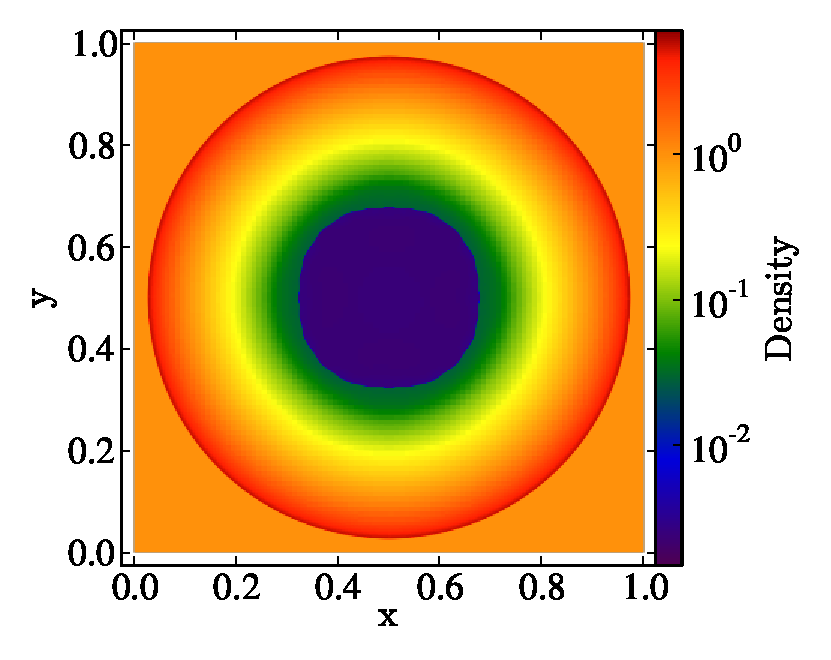
\includegraphics[width=0.4\textwidth]{figures/sedov-ppm-slice.eps}
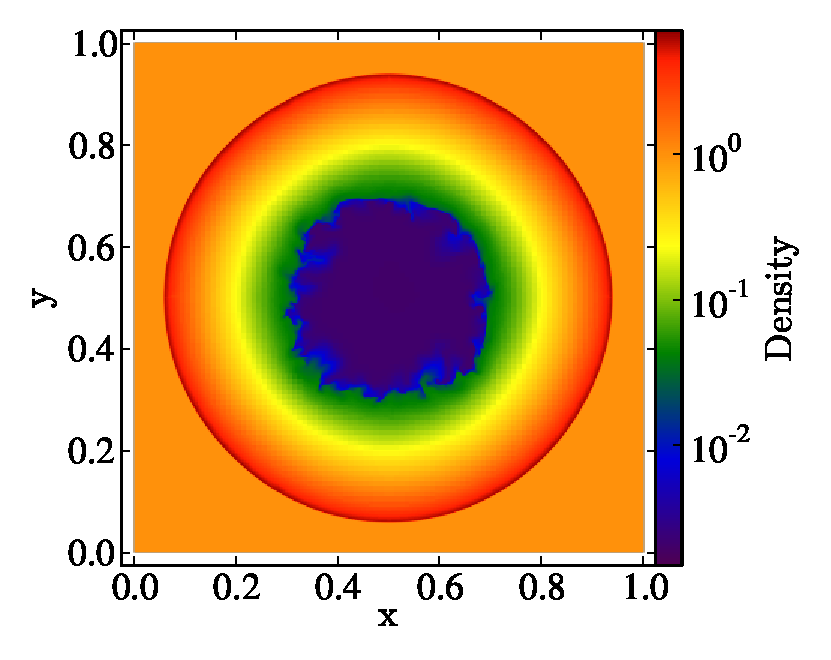
\includegraphics[width=0.4\textwidth]{figures/sedov-zeus-slice.eps}
\caption{Density slice from the Sedov Blast test at $t = 0.07$. Left:
results using the Piecewise Parabolic Method hydro scheme.  Right: results using the \zeus\
hydro method. Notably, the \zeus\ shock front has progressed less far
than in the PPM run. This is due to energy loss when conserving only
internal, and not total, energy.}
\label{fig.sedov1}
\end{center}
\end{figure}


\begin{figure}
\begin{center}
\includegraphics[width=\textwidth]{figures/sedov-profiles.eps}
\caption{Radially averaged profiles for the Sedov Blast test at $t =
0.07$. Clockwise from top-left shows density, velocity, internal
energy and pressure.  The black solid line shows the analytic
solution.  The blue dashed line shows the simulation using the PPM
method, and the red dot-dashed line using \zeus.  The \zeus\ result
substantially lags the true result due to total energy not being
explicitly converged.}
\label{fig.sedov2}
\end{center}
\end{figure}

The Sedov Blast Test \citep{Sedov1959} models an intense explosion,
initiated by depositing thermal energy into a homogenous distribution
of gas. The result is a strong spherical shock wave centered on the
point of energy injection.  This problem is a popular test of
astrophysical numerical codes for three reasons: First, it is
particularly appropriate to astrophysics since it represents the
situation when a supernovae explosion occurs. Second, it has an
exact analytical solution whereby the shock front's radial position is
given by:

\begin{equation} r(t) =
\left(\frac{E_0}{\alpha\rho_0}\right)^{1/5}t^{2/5}
\end{equation}

\noindent where $E_0$ is the initial energy injection, $\rho_0$ is the
background density and $\alpha = 1.0$ for cylindrical symmetry and an
ideal gas with $\gamma = 1.4$. For the full derivation see
\citet{Sedov1959}. This solution makes it possible to assess how well
the code performs.  Third, the spherical shock is a challenging
problem for numerical codes (both grid and particle) since the shock
wave increases in size as the simulation progresses and its
symmetrical nature highlights any directional preferences that grid
codes can succumb to. The test presented here is the two-dimensional
version that is included in the \enzo\ distribution. The
three-dimensional results from this test, both for \enzo\ and three
other leading astrophysics codes, can be founds in \citet{Tasker2008}.

In the initial state, the box contains a homogenous distribution of
gas at a density of 1 (note that, in the absense of gravity, this
problem is scale-free and thus without units). Thermal energy is
deposited into a single cell at the center of the box with $E_0 =
10.0$. The problem is completed in two dimensions with reflecting
boundary conditions (the default for \enzo) and uses a box size of side
$1$. For this problem, we selected a top grid of $100 \times 100$
cells and a maximum of four levels of refinement, placed based on
shock location and the slope in density and total energy. The
exception to this scheme is in the initial conditions, where grids are
placed directly around the injection point. The results were assessed
at $t = 0.07$, which corresponding to a time just before the shock
reaches the box edge (see Figure~\ref{fig.sedov1}).

Figure~\ref{fig.sedov2} shows the radial profiles for the simulation
run with the PPM hydro-solver (blue dashed line) and the \zeus\
hydro-solver (red dash-dot-dot line) together with the analytical
solution (black solid line). Clockwise from the top-left are density,
velocity, internal energy and pressure. PPM matches the analytical
solution extremely well for all quantities. However, the shock front
in the \zeus\ simulation lags behind the analytical position. This can
also be seen in the slices shown in Figure~\ref{fig.sedov1}. The cause
of this discrepancy is that \zeus\ shows a substantial energy loss
during the first few timesteps and produces a diamond-shaped, rather
than spherical, shockfront during this time. After this, the code
correctly conserves energy but this intial energy loss remains clearly
visible in the position of the shock at $t = 0.07$. This problem was
addressed directly by \citet{Clarke2010}, who attributed the source of
the issue to this version of \zeus\ solving the internal, rather than
total, energy equation. In situations with strong energy gradients,
this choice caused an energy loss and the artificial viscosity
produces the direction-dependent shockfront shape. In their paper,
\citet{Clarke2010} presents results from an alternative version of
\zeus\ that conserves total energy. This problem is less marked for
smaller energy gradients and it should be noted that the \zeus\ hydro
algorithm's stability and speed make it a highly competitive choice,
despite the disagreements in this test.


%%%%%%%%%%%%%%%%%%%%%%%%%%%%%%%%%%%%%%%
\subsubsection{Point source gravity test}
\label{sec.test.gravitypointsource}
\red{(Greg)}
This is the TestGravity (problem 23) test problem.  It tests gravity around a point source, using fixed AMR.

%%%%%%%%%%%%%%%%%%%%%%%%%%%%%%%%%%%%%%%
\subsubsection{Orbit Test}
\label{sec.test.testorbit}
\red{(Greg)}
This is the TestOrbit problem (problem 29 for GB).  This tests gravity and particle integration (no hydro).

%%%%%%%%%%%%%%%%%%%%%%%%%%%%%%%%%%%%%%%
\subsubsection{Self-Similar infall test}
\label{sec.tests.infall}
\red{(Greg)}
Problem type 24.  This is a test based on Bertschinger's 1985 3D self-similar infall
solution, and tests gravity + hydro.

%%%%%%%%%%%%%%%%%%%%%%%%%%%%%%%%%%%%%%%
\subsubsection{Zel`dovich Pancake}
\label{sec.tests.pancake}

The Zel`dovich pancake \citep{1970A&A.....5...84Z} is particularly
relevant to cosmological simulations, because it includes many
features that are critical to structure formation: hydrodynamics,
expansion, and self gravity.  This problem represents the formation of an ideal,
isolated caustic, and is thus a useful proxy for much more
complicated structures in full 3-dimensional cosmological simulations
(such as the collapse of gas onto a cosmological halo or filament).

The initial conditions are simple, and we follow the prescription of
\citet{Anninos94}.  Assuming a geometrically flat cosmology, the density
perturbation is given by

\begin{equation}
\rho(x_l) = \rho_0 \big[ 1 - \frac{1+z_c}{1+z} \cos(k x_l) \big]
\end{equation}

with the internal energy of the gas set so that the entropy of the gas
maintains a constant value throughout.  The velocity perturbation is given by

\begin{equation}
v(x_l) = -H_0 \frac{1 + z_c}{(1+z)^{1/2}} \frac{\sin(k x_l)}{k}
\end{equation}

In the equations above, $\rho_0$ is the background density, z$_c$ is a
free parameter and is the redshift where the sheet forms a caustic
(i.e., where it `pancakes'), z is the redshift of initialization, x$_l$ is the
Lagrangian mass coordinate, $k = 2 \pi / \lambda$ (where $\lambda$ is
the perturbation wavelength), and H$_0$ is the $z = 0$ value of the
Hubble constant.  Note that this solution is expressed in terms of
Lagrangian positions, so one needs to convert this into the Eulerian
coordinates, x$_e$, that are more useful to \enzo:

\begin{equation}
x_e = x_l - \frac{1 + z_c}{1 + z} \frac{\sin(k x_l)}{k}
\end{equation}

We note that the solution described above is exact up to the point of
caustic formation.  In Figure~\ref{fig.pancake}, we show the results
of a test of the adaptive mesh version of \enzo's Zel'dovich Pancake test.  A
one-dimensional box of length $64$~Mpc/h is initialized at z$ = 20$ in
an $\Omega_M = 1$ universe with h$ = 0.5$ and a background temperature
of 100~K, $\rho_0 = \rho_c$.  The simulation is initialized with 64
grid cells, refining by factors of four using criteria based on cell
mass and the presence of shocks, for a maximum of 2 levels (i.e., an
equivalent maximum resolution of 1024 grid cells).  The simulation was
evolved to z$ = 0$ using the PPM hydro method, with the final output
of the calculation being shown in Figure~\ref{fig.pancake}.

Figure~\ref{fig.pancake} shows the key features of this test problem.
The strong shocks and large density gradients are well-resolved, with
density and velocity jumps being well-delineated and at the correct locations.  The key features of
this test problem can be resolved with far fewer cells -- simulations
including a mere 8 cells resolve the key features, as shown in
Sections 3.3.4-3.3.5 of~\citet{1996PhDT........80B} -- but we choose a
higher resolution here for illustrative purposes.

\begin{figure}
\begin{center}
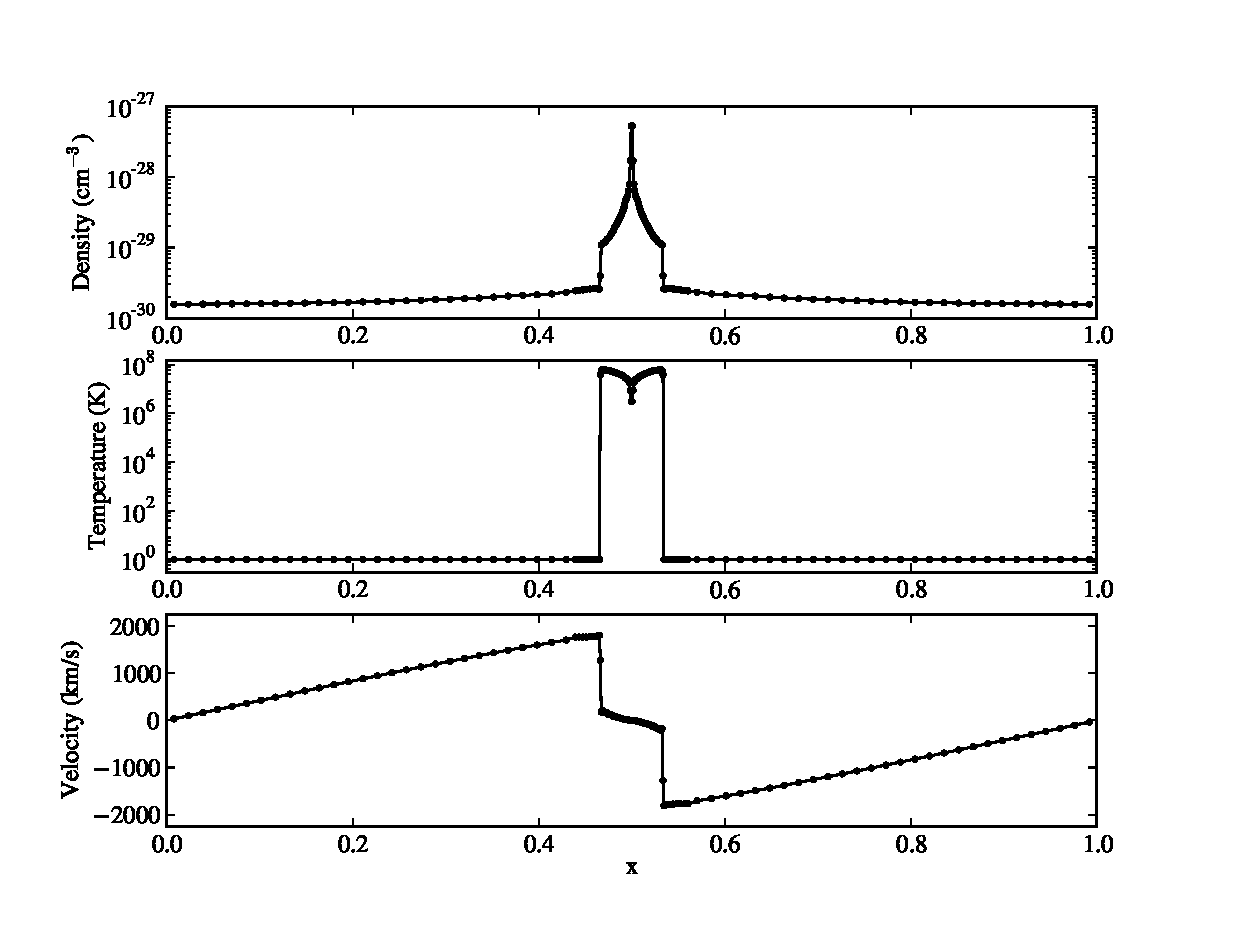
\includegraphics[width=0.8\textwidth]{figures/AMRZeldovichPancake.eps}
\caption{Zel`Dovich Pancake test shown at z$ = 0$, initialized in a
$\Omega_m = 1$ universe at z$ = 20$ on a one-dimensional grid having
64 cells, and further refined by factors of four based on cell mass
and the presence of shocks for up to two additional levels of mesh,
having a maximum effective resolution of 1024 grid cells. The top,
middle, and bottom rows show density, temperature, and velocity of the
gas, respectively; all are a function of position in units of the box
size.  The central region ($x \simeq 0.45-0.55$) has bene adaptively
refined, as can be seen by the locations of grid points.  Shocks and
the central density peak are clearly resolved, with well-delineated
jumps at the appropriate locations.}
\label{fig.pancake}
\end{center}
\end{figure}


%%%%%%%%%%%%%%%%%%%%%%%%%%%%%%%%%%%%%%%
\subsubsection{MHD: Orszag-Tang Vortex}
\label{sec.tests.mhd}
Figure~\ref{fig.orszag} shows the Orszag-Tang vortex problem, a
standard magnetohydrodynamic test problem \citep{Orszag79}.  The left panel shows
the result using \enzo's constrained transport MHD method, while the right panel shows the result using
\enzo's implementation of Dedner MHD.
The Orszag-Tang vortex test shows that significant small scale structure can be generated in MHD
from large scale initial perturbations, and is used to compare the
effective resolution of different MHD schemes.  The test begins with uniform
density, $\rho_0=25/36 \pi$ and pressure, $P_0=5/12 \pi$ (as with
other tests in this section, in the absence of gravity or chemistry we use
arbitrary units).  There is a
single rotational mode in the velocity, and two in the magnetic field:
${\bf v}_0 $ = (-sin(2$\pi$ y) $ \hat{x}$ , sin(2$\pi$ x) $\hat{y}$),
${\bf B}_0$ = (-sin(2 $\pi$ y) $ \hat{x},$ sin( 4 $\pi$ x )$\hat{y}$).
The simulation is evolved to $t=0.48$ (in arbitrary units).  One can see that the structures
are accurately represented as compared to, for instance,
\citet{Toth00}, and that the resolution of shocks is comparable in
both methods.

\begin{figure}
\begin{center}
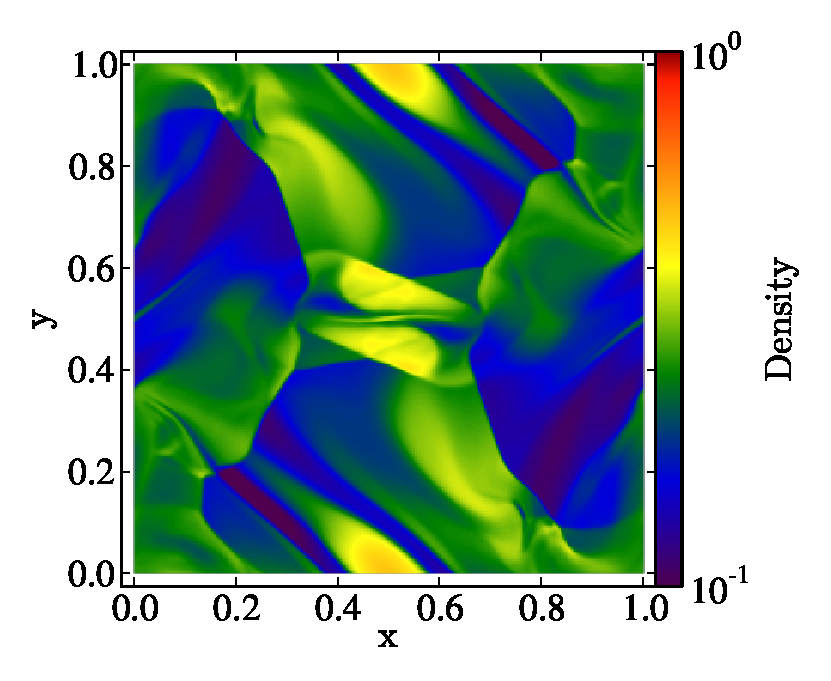
\includegraphics[width=0.4\textwidth]{figures/MHDCT_OrszagTang_Density.eps}
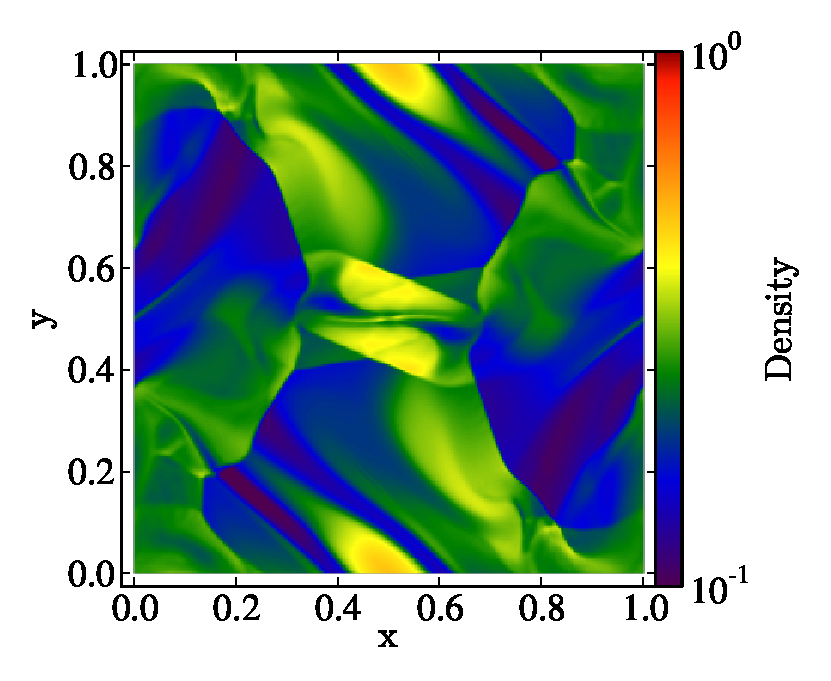
\includegraphics[width=0.4\textwidth]{figures/MHDDedner_OrszagTang_Density.eps}
\caption{Density field from the Orszag-Tang vortex test, at $t=0.48$.
Left: solution using constrained transport MHD.  Right: solution using
Dedner MHD. The initial conditions are uniform density, with a single
rotating velocity structure and two circular magnetic structures.
These initial conditions generate significant small-scale structure in
both the CT and Dedner schemes, which have approximately equal
effective resolution.}
\label{fig.orszag}
\end{center}
\end{figure}


%%%%%%%%%%%%%%%%%%%%%%%%%%%%%%%%%%%%%%%
\subsubsection{One-zone collapse test}
\label{sec.tests.1-zone}

The one-zone collapse test simulates the collapse of a
self-gravitating gas cloud using a semi-analytic model for the
evolution of gas density and adiabatic heat input as a function of
time.  It is designed to test the chemistry and cooling modules over a
wide range in densities and over physically motivated timescales.
Because this test disables the hydrodynamic and gravity solvers and
uses a simple model for the density evolution, it is far faster than
running a true collapse simulation.  The density evolution is based on
the self-similar Larson-Penston \citep{1969MNRAS.145..271L,
1969MNRAS.144..425P} solution for isothermal collapse with a
modification to account for the efficiency with which the heat
introduced by compression can be radiated away
\citep{1983ApJ...265.1047Y}.  Our implementation, described briefly
here, follows the work of \citet{2005ApJ...626..627O}, and we direct
the interested reader to this paper for further details.  The
evolution of the gas density, $\rho$, is given by

\begin{equation}
\frac{d\rho}{dt} = \frac{\rho}{t_{col}},
\end{equation}

where the collapse timescale, $t_{col}$, is

\begin{equation} \label{eqn.tcol}
t_{col} = \frac{t_{dyn}}{\sqrt{1 - f}},
\end{equation}
In this equation, $t_{dyn}$ is the dynamical time and is expressed as
\begin{equation}
t_{dyn} = \sqrt{\frac{3 \pi}{32 G \rho}}.
\end{equation}

with G being the gravitational constant.  The collapse timescale is
altered from the dynamical time by a factor $f$ in Equation
\ref{eqn.tcol}, which is an approximation of the ratio of the gas
pressure to the force of gravity.  The value of $f$ depends on the
effective adiabatic index, $\gamma_{ef} \equiv (\partial ln\ p
/ \partial ln\ \rho)$, which we calculate by linearly extrapolating
from derivative values for the two previous timesteps.  For the value
of $f$ in this test problem, we use the piecewise function of
\citet{2005ApJ...626..627O}, given by

\begin{equation}
f = \left\{
  \begin{array}{ll}
  0, & \gamma_{ef} < 0.83,\\
  0.6 + 2.5 (\gamma_{ef} - 1) - 6.0 (\gamma_{ef} - 1)^{2}, & 0.83 <
  \gamma_{ef} < 1,\\
  1.0 + 0.2 (\gamma_{ef} - 4/3) - 2.9 (\gamma_{ef} - 4/3)^{2}, & \gamma_{ef} > 1.
\end{array} \right.
\end{equation}

The specific energy evolves as

\begin{equation}
\frac{de}{dt} = -p \frac{d}{dt} \frac{1}{\rho} - \Lambda,
\end{equation}

where $\Lambda$ is the cooling rate in units of erg s$^{-1}$ g$^{-1}$
and energy, temperature, density, and pressure are related by the
ideal gas law.  Figure \ref{fig.onezone} shows an example of the
one-zone collapse test performed with an initial number density of 1
hydrogen atom per cm$^{-3}$ and an initial temperature of 100 K using
the 12 species chemistry network with H, D, and He species and metal
cooling rates calculated with the \texttt{Cloudy} code.  The effects
of metal cooling can be clearly seen; as the metallicity increases
from zero to $10^{-2}$~Z$_\odot$, the gas deviates from the primoridal
result (black line) both more rapidly and more significantly.  Our
primordial results compare very well to those shown in
\citet{2005ApJ...626..627O}; however, we use a different cooling
method than Omukai, so the lines describing the evolution of the
metal-enriched gas are not directly comparable.

\begin{figure}
  \begin{center}
    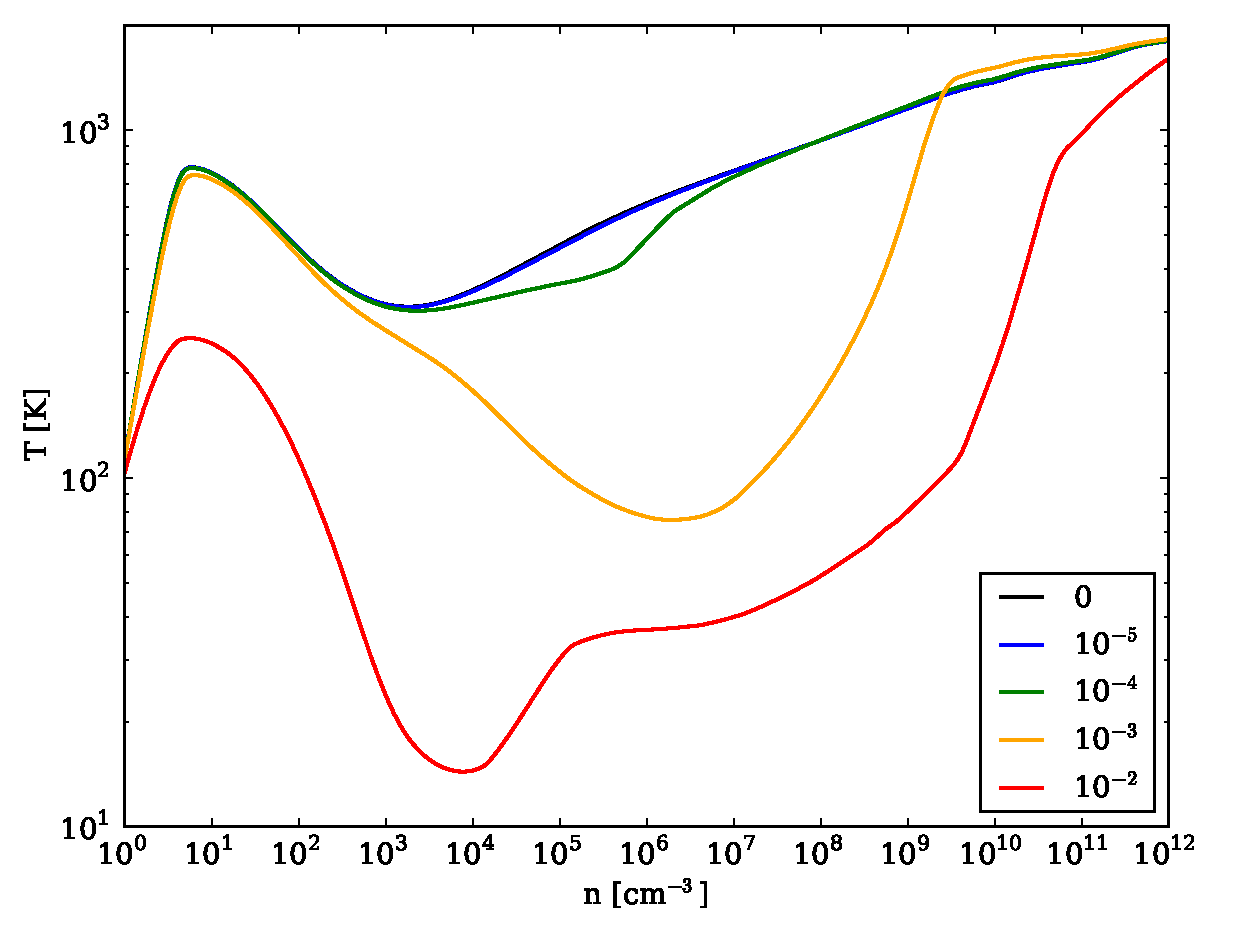
\includegraphics[width=1.0\textwidth]{figures/OneZoneCollapseTest.eps}
  \end{center}
  \caption{Evolution of temperature versus number density for a
one-zone collapse test for gas at metallicities from 0 to 10$^{-2}
Z_{\odot}$.  This test is based on the results of
\citet{2005ApJ...626..627O}, and approximates the collapse of a
self-gravitating, cooling gas cloud.  This test problem uses \enzo's
primordial chemistry network with tabulated metal cooling rates
calculated with the \texttt{Cloudy} code, and compares favorably to
Omukai's results.}
  \label{fig.onezone}
\end{figure}


%%%%%%%%%%%%%%%%%%%%%%%%%%%%%%%%%%%%%%%
\subsubsection{Photo-evaporation of a dense clump}
\label{sec.tests.raytracing}

The photo-evaporation of dense clumps of gas is prevalent in radiation
hydrodynamics simulations, and this test problem examines the
ionization front propagation into the dense clump, shadowing effects
behind the clump, and the hydrodynamic response on the clump from
photo-heating, all using \enzo's Moray ray-tracing module.  The
problem setup is the same as Test 7 in the Cosmological Radiative
Transfer Comparison Project \citep{IlievEtAl2009} and
\citet{Wise11_Moray}.  The simulation domain is 6.6~kpc on a side with
an ambient medium of pure neutral hydrogen $n_{\rm H} = 2 \times
10^{-4}\; \cubecm$ and $T = 8000 \unit{K}$.  We place a spherical
overdensity in hydrostatic equilibrium with the ambient medium.  It
has a radius $r = 0.8 \unit{kpc}$, hydrogen density $n_{\rm H} = 0.04
\cubecm$, and temperature $T = 40$ K, and it is centered at $(x,y,z) =
(5, 3.3, 3.3) \unit{kpc}$.  In \citet{IlievEtAl2009}, all of the codes
used a fixed $128^3$ grid to ease the comparison, but in this test to
demonstrate a higher resolution AMR solution, we employ a $128^3$ grid
with two additional levels of refinement with cells with a baryon mass
(method 2 in Section~\ref{sec:refinement_criteria}) greater than 1.5
being flagged for refinement.  This test is run for 15 Myr.

This cloud is subject to radiation from a point source at the center
of the $y=0$ boundary with an ionizing photon luminosity
$\dot{N}_\gamma = 3 \times 10^{51}$ photons s$^{-1}$, corresponding to
a flux $F_0 = 10^6 \unit{photons s}^{-1} \unit{cm}^{-2}$ at the clump
surface closest to the radiation source.  The radiation source has a
spectrum of a $T = 10^5 \unit{K}$ blackbody, and we use four energy
groups with the following mean energies and relative luminosities:
$E_i = (17.98, 31.15, 49.09, 76.98) \unit{eV}, L_i/L = (0.23, 0.36,
0.24, 0.06)$ that are optimized to reduce errors in the solutions with
a full spectrum and energy discretization \citep{Mirocha12}.
\citep[Note that this choice of energy groups is different
from][]{Wise11_Moray}.  We use a minimum angular resolution of 10 rays
per cell and a constant radiative transfer timestep of 25 kyr.  Figure
\ref{fig:shadowing} depicts the clump after at $t = 15$ Myr with the
outer layers expanding after being photo-heated.  It also shows the
sharp shadowing effects of the dense clump in the neutral fraction
plot that is representative of ray tracing techniques.

\begin{figure}
  \centering
  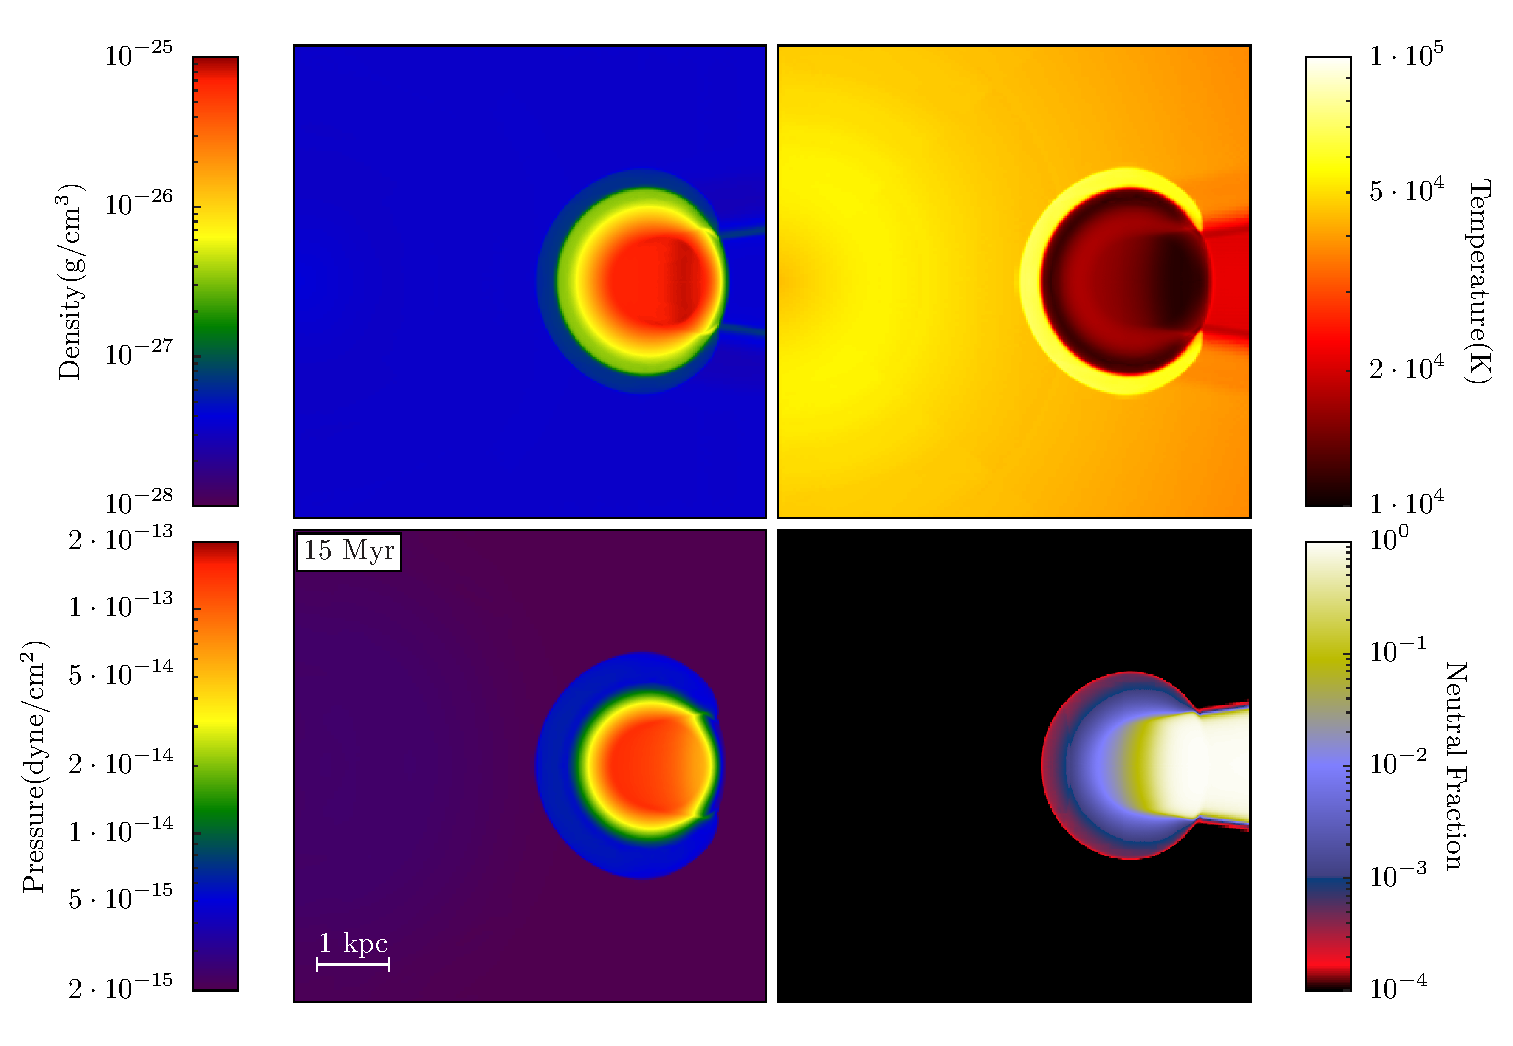
\includegraphics[width=1.0\textwidth]{figures/code-test-shadowing.eps}
  \caption{Photo-evaporation of a dense clump using the Moray
ray-tracing module.  Clockwise from the upper left corner: slices
through the clump center of the density, temperature, neutral hydrogen
fraction, and pressure at $t=15$~Myr after the initialization of the
simulation.  A point source of radiation is at the center of the -x
boundary and illuminates the clump with a constant luminosity, casting
a clear shadow behind the clump, as seen in the neutral hydrogen
fraction.}
  \label{fig:shadowing}
\end{figure}

%%%%%%%%%%%%%%%%%%%%%%%%%%%%%%%%%%%%%%%
\subsubsection{Representative FLD test}
\label{sec.tests.fld}

\red{(Dan)}
One test for the implicit FLD: best/hardest one.



%%%%%%%%%%%%%%%%%%%%%%%%%%%%%%%%%%%%%%%

\subsubsection{Anisotropic Thermal conduction}
\label{sec.tests.conduct}

In a plasma, conduction takes place primarily due to electron motion.
In astrophysical environments such as the intergalactic and
intracluster media, with typical magnetic strengths of $\sim 1$~$\mu$G
and temperatures in the millions of Kelvin, the electron gyroradius is
very small compared to the scales of interest in a typical
cosmological simulation.  As a result, electrons can only move
\textit{along} magnetic field lines, not perpendicular to them, which
can result in very interesting magnetohydrodynamical instabilities
\citep[e.g.,][]{2008ApJ...677L...9P,2008ApJ...688..905P}.  The correct
modeling of this behavior can be quite challenging, and is described
in Section~\ref{sec.num.conductions}.  Conduction in \enzo\ is
calculated in both an operator-split and directionally-split manner,
and the addition of heat transport solely along magnetic field lines
requires computation of cross-terms in the temperature derivative at
cell faces, which can add spurious oscillations in the temperature
field in regions where the temperature gradient is strong in more than
one spatial direction unless an appropriate flux-limiter \citep[such
as that of][]{1977JCoPh..23..263V} is chosen.

Figure~\ref{fig.conduct} shows a test that demonstrates the correct
behavior of anisotropic thermal conduction in \enzo.  We initialize a
two-dimensional, $256 \times 256$ cell simulation having a physical
scale of 1 kpc on a side, a uniform density of 1 proton/cc, and a
background temperature of $10^6$ Kelvin.  Magnetic fields with a
strength of B$_0 = 1$~$\mu$G are initialized such that the field lines
form circles around the center of the simulation volume, such that
B$_x = -B_0\sin(\theta)$ and B$_y = B_0\cos(\theta)$, where $\theta$
is the angle measured from the $+x$ direction in a counterclockwise
manner.  A Gaussian temperature pulse is injected at $(0.75, 0.5)$ (in
units of the box size), with a peak temperature of $10^8$ K and a FWHM
of $1/64$ of the box size.  This initial setup is shown in the left
panel of Figure~\ref{fig.conduct}.  The simulation is then allowed to
evolve with \textit{only} anisotropic conduction turned on (e.g., no
hydrodynamics, radiative cooling, or cosmological expansion), and with
a Spitzer fraction of f$_{sp} = 1$.

The right panel of Figure~\ref{fig.conduct} shows the state of the
simulation after 300 Myr.  Heat has clearly been transported only along
field lines -- there has been no diffusion perpendicular to the
magnetic field setup, which is critical for many studies involving
anisotropic thermal conduction.  No oscillations are seen in the
temperature field in regions where the fields are not aligned with the
grid, suggesting that the flux-limiter is operating as expected.

\begin{figure}
\begin{center}
\includegraphics[width=0.42\textwidth]{figures/aniso_conduction_initial_output.eps}
\includegraphics[width=0.4\textwidth]{figures/aniso_conduction_final_output.eps}
\caption{Two-dimensional anisotropic conduction test in a uniform,
constant temperature background with circular magnetic fields centered
on (0.5, 0.5) in a $256 \times 256$ grid.  The background medium has a
density of 1 proton/cc and a temperature of $10^6$~K.  At t$ = 0$
(left panel), a Gaussian heat pulse is injected at (0.75, 0.5) with a
FWHM of $1/64$ (with all numbers given in units of the box size) and a
peak temperature of $10^8$~K, and allowed to evolve without
hydrodynamical motion (i.e., static gas) and no radiative cooling for
300 Myr.  At t$ = 300$~Myr (right panel), heat has been transported
along magnetic field lines with no significant diffusion perpendicular
to field lines. Furthermore, there are no detectable oscillations in
the temperature in regions where the magnetic field is not parallel
with the grids.}
\label{fig.conduct}
\end{center}
\end{figure}


%%% Local Variables: 
%%% mode: latex
%%% TeX-master: "ms"
%%% End: 
